
\documentclass[tikz]{standalone}

\begin{document}
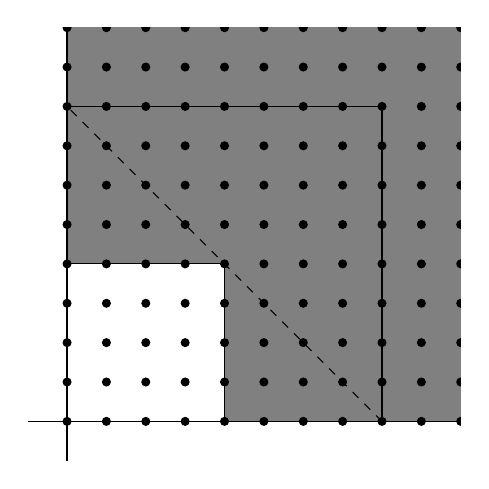
\begin{tikzpicture}
  \clip (-0.5, -0.5) rectangle (5, 5);
  \draw[fill=gray] (0, 0) rectangle (5.2, 5.2); 
  \draw[fill=white] (0, 0) rectangle (2, 2);
  \draw (-0.5, 0) -- (5, 0);
  \draw (0, -0.5) -- (0, 5);
  \draw[dashed] (4, 0) -- (0, 4);
  
  \foreach \x in {0, 0.5, ..., 5} {
    \foreach \y in {0, 0.5, ..., 5} {
  \draw[fill=black] 
  (\x, \y) circle
    (0.05);
  }
}


\draw (0, 4) -- (4, 4) -- (4, 0);




\end{tikzpicture}
\end{document}
